\documentclass[11pt]{article}
\usepackage[utf8]{inputenc}
\usepackage[margin=1.0in]{geometry}
\usepackage{graphicx}
\usepackage{wrapfig}
\usepackage{amsmath}
\usepackage{caption}
\usepackage[makeroom]{cancel}
\usepackage{hyperref}
\usepackage{listings}
\let\vec\mathbf

\title{Convolutional Neural Nets 2}
\author{Neal Bayya}
\date{February 27, 2019}

\begin{document}

\maketitle

\section{Review of Theory}
\subsection{Neural Network Basics}
Regular Neural Networks (sometimes referred to as "vanilla neural networks") have an input layer which is a single vector followed by a series of linear transformations through hidden layers separated with non-linear activation functions. Examples of such functions include the sigmoid function, hyperbolic tangent function, and ReLU. The values at these hidden layers are not important and only serve to store data as the input is transformed into the output vector. Regular Neural Networks do \textit{not} scale well to images because the number of parameters we would have to tune grows quickly. 
\subsection{Convolutional Neural Network}
With the high dimensionality of images, it is not practical to connect each node in the flattened image vector with all other nodes as is done in regular neural networks. Convolutional neural networks provide a more sensible way to process image data. Instead of sequentially transforming the input through layered vectors as in regular neural networks, convolutional nets transform the input through sequences of 3 dimensional tensors \footnote{A tensor is a generalization of vectors and multidimensional arrays to arbitrary shapes. }. Each node in a particular tensor will only connects nodes from a localized region in previous tensor to preserves spatial information and reduce the number of parameters needed. Similar to Regular Neural Networks, Convolutional Neural Networks can be decomposed into a sequence of layers. Recall the \textit{four main layers} that are used in constructing Convolutional Neural Networks (by no means are these the only types):
\begin{enumerate}
    \item \textit{Convolution Layers:} The parameters in the Conv layer consist of a set of filters. The filters are small in width and height (typically 3x3 or 5x5) but extend to the full depth of the input volume. When we slide a filter over the input volume, we get a 2-D activation map. The output of the Conv layer is a 3-D stack of the activation maps produced by each of the filters.  It is important to note that these filters are not inputted as hyper-parameters but are instantiated randomly and learned through backpropogation. The hyper-parameters to the Conv layer include the size of each kernel as well as the number of kernels.
    \item \textit{Pooling Layers:} Pooling layers are often used between successive Conv layers to reduce the width and height of the tensor that is processed. Max pooling is the most common form of pooling in which each 2-D map of the input tensor is sub-sampled by taking the maximum intensity from each $n \times n$ patch. The patch size, $n$, would be a hyperparameter inputted by the user in creating the model. In reducing the dimensionality of our data, pooling layers reduce the amount of parameters and computation that goes on in the network. A common misconception is that the reduction in computational burden comes at the cost of CNN accuracy. However, pooling layers are actually very important to prevent overfitting because we are "forcing" the CNN to store the same information in a more compact structure. 
    \item \textit{ReLU Layer:} Recall that the ReLU function for input $x$ is $max(0,x)$. The function is applied element wise on the input tensor. This layer is often built into the Conv layers in many popular machine learning packages such as Keras. ReLU is the most common activation function that is used in CNNs. It is difficult to give mathematical justification for why it works best, but it just has worked best in practice. 
    \item \textit{Fully Connected Layer:} To complete the task of classification, most CNNs typically use dense layers, or fully connected layers. These terms both refer to the connection layers found in typical neural networks, mainly to distinguish them from other layers (convolutional, pooling).
\end{enumerate}

\begin{figure}
    \begin{center}
        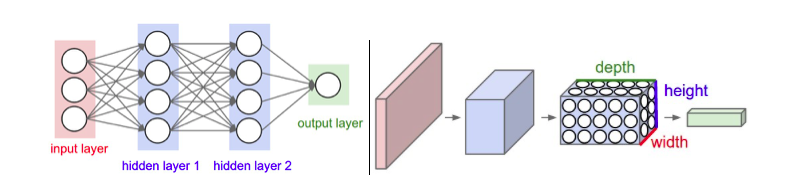
\includegraphics[width=\textwidth]{layers.png}
        \vspace{-10pt}
        \caption{Left: A 3 layer neural network. Right: A Conv Net which maintains the 3-D structure of the image through each layer. The red tensor represents the input image and the subsequent tensors are generated through conv layers.}
    \end{center}
    \vspace{-25pt}
\end{figure}


\section{CNN Usage in Practice}
There are still many more layer types or modifications that can be made to CNN design. We have barely scratched the surface. For example, machine learning libraries offer functionality with normalization layers, layer concatenations (in which you could train multiple networks and combine them), etc. It is easy to get overwhelmed by the amount of different architectural designs that are available when constructing a CNN. Lucky for us, most applications do not require such complex structures. Stanford's CS231 Course (which I highly recommend), put's it nicely as "Don't be a hero. Instead of rolling your own architecture for a problem, you should look at whatever architecture currently works best on ImageNet, download a pretrained model and finetune it on your data." After reading through Section 2, try to wrap your head around Figure \ref{VGG}, which outlines the layers of the popular VGG Convolutional Neural Network.

\subsection{Layer Patterns}
The most common format for a CNN starts with multiple Conv-ReLU layers, follows with a pooling layer, and repeats the pattern until the tensor is reduced to a small size. After reaching the small size, the tensor is flattened into a vector, and fully-connected layers are used. The output layer is the final layer of the fully-connected layer. The following expression describes the general CNN architecture more succinctly: \\
\begin{center}
$INPUT \longrightarrow \left[\left[ CONV \longrightarrow RELU \right]^*N \longrightarrow POOL? \right]^* M \longrightarrow \left[ FC \longrightarrow RELU \right]^*K \longrightarrow OUTPUT $
\end{center}
where the * superscript indicates repetition and the POOL? indicates an optional pooling layer. Below is a general rule of thumb for what values to choose for N, M, and K.
\begin{itemize}
    \item $\mathbf{0 \leq N \leq 3}$ \quad Multiple stacked Conv layers will help extract more complex features before information is lost through pooling.
    \item $\mathbf{M \geq 0}$ \quad $M = 0$ just represents a regular neural network. As a result you can think of regular neural networks as subsets of CNNs. An upper bound is not provided because you should keep applying the CONV-RELU and POOL block until your tensor is sufficiently small. How small, you may ask? You will have to play around with this value because there is no definite answer. 
    \item $\mathbf{0 \leq K \leq 2}$ \quad Dense layers are computationally expensive to train, so don't add too many. Plus, if you have pooled your data enough, then you should not need that many to begin with.
\end{itemize}
\textbf{Note on Filter Sizes}: Smaller filters outperform those which have a larger receptive field (larger height and width). Let's say that you stack 3 CONV-RELU layers, where each CONV layer uses a filter size of $3 \times 3$. A node in the first CONV layer will express a $3 \times 3$ window of the input image. A node in the second CONV layer will express a $3 \times 3$ window of the first CONV layer and thus a $5 \times 5$ window of the input image. No, it is \textit{not} a $9 \times 9$ window of the input image because convolutions happen over a sliding window as opposed to over discrete patches. Now, here is the question we have been building towards: Why not use a $5 \times 5$ filter in the first CONV layer as opposed to stacking two $3 \times 3$ type CONV layers? After all, they have the same receptive field on the input image. The answer is that stacking CONV layers with smaller receptive fields is preferable because the layers are separated with non-linearities which make the features more meaningful. Further, the single $5 \times 5$ CONV approach consumes $C \times \left( 5 \times 5 \times C \right)$, whereas the stacked CONV approach only uses $2 \times \left( C \times \left( 3 \times 3 \times C \right) \right)$ parameters, assuming all of the tensors have a depth of $C$.

\begin{figure}
    \begin{center}
        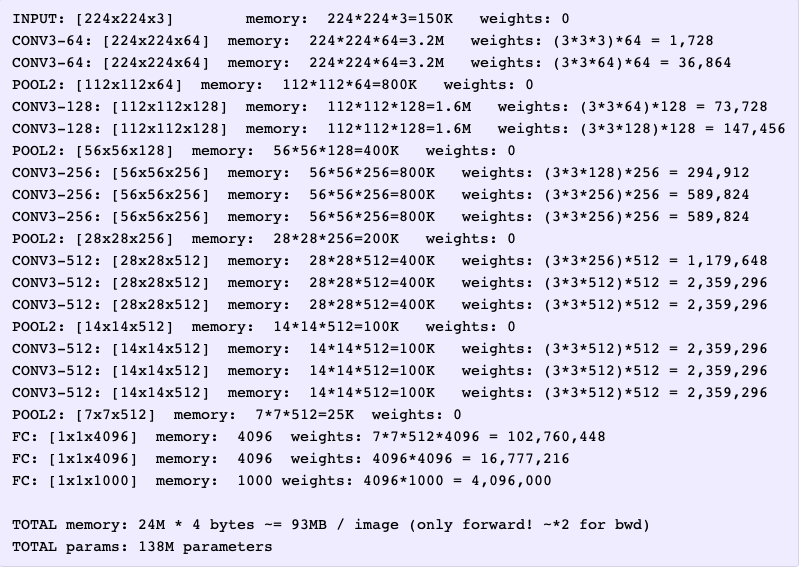
\includegraphics[width=0.5\textwidth]{VGG.png}
        \caption{A layer by layer breakdown of VGG16. The main contribution of VGG net in the ImageNet competition was demonstrating the importance of having a deep neural network. A pretrained VGG net is loaded in most popular deep learning libraries for transfer learning, which is just the process of re-training a pretrained model for a new task.}
        \label{VGG}
    \end{center}
\end{figure}

\subsection{Layer Sizing}
Below are some additional notes that you should keep in mind when deciding the sizes of your variables in your CNN architecture. \\
\textbf{Input: }Try to make the width and height of your image divisible by 2 many times. This can often be achieved by taking $n \times n \times 3$ sized crops of your image, where common values of n include 128, 224, 284, and 512. \\
\textbf{CONV Layers} As mentioned in subsection 2.1, use $3 \times 3$  filter sizes. Additionally, it will save you many headaches if you use padding in the CONV layer such that the height and width of the tensor stay the same. Save the compression for pooling. The proper padding amount is related to the filter size through the following relationship: $P = (F-1)/2$. \\
\textbf{POOL Layers:} The most common setting for pooling layers it to do MAX pooling with $2 \times 2$ receptive fields and a stride of 2. Be very cautious when increasing the receptive field because the amount of lost information increases in a quadratic manner. If you are increasing the size of the receptive field, make sure that you have many CONV layers preceding it. 

\section{Keras Implementation}
\subsection{Intro to Keras}
Keras is a high-level machine learning library that makes it very easy to construct neural networks or work with pre-trained models such as VGG16 or ResNet. Keras is built over other lower-level machine learning libraries such as Theano or Tensorflow and is optimized for fast experimentation. Further, Keras is optimized for the GPU as well as CPU because its internal matrix operations use CuDNN, which parallelizes the computation. You can install Keras with the command: \texttt{pip3 install keras}. I recommend using Keras along with libraries such as \texttt{numpy} and \texttt{pandas}, which help with fast numerical operations and data preprocessing, respectively.

\subsection{Building Models}
We will build a CNN for the MNIST dataset, in which we were classifying hand-written digits.

\begin{lstlisting}
import numpy as np
import keras
from keras.datasets import mnist
from keras.models import Sequential
from keras.layers import Dense, Dropout, Flatten
from keras.layers import Conv2D, MaxPooling2D
from keras.optimizers import Adam, SGD
\end{lstlisting}

\texttt{keras.datasets} contains many datasets such as cifar100 and mnist so that you will not have to load them yourself. \texttt{keras.models.Sequential} is a tool that we will use to stack a sequence of layers which will make up our neural network. These layers, which are defined in \texttt{keras.layers}, each come have methods for feeding the nueral network forward through the layer and calculating the gradient through for backpropogation. When we stack these layers in \texttt{Sequential{}}, keras combines the feedforward methods as well as the backpropogation methods, so the user does not have to worry about these things. \texttt{keras.optimizers} includes support for algorithmic additions to standard backpropogation which often result in faster learning or less overfitting.

\begin{lstlisting}
#Define our hyper-parameters
nonlin = 'relu'
epochs = 15
num_classes = 10
batch_size = 128

#Load data and pre-preprocess
(x_train, y_train), (x_test, y_test) = mnist.load_data()
x_train = x_train.reshape(x_train.shape[0], 28, 28, 1) #28 x 28 images
x_test = x_test.reshape(x_test.shape[0], 28, 28, 1) 
x_train = x_train.astype('float32')
x_test = x_test.astype('float32')
x_train /= 255
x_test /= 255
\end{lstlisting}

 The imported mnist dataset will give us 6000 samples in our train set and 1000 samples in our test set. We keep the input shape to our model as $28 \times 28 \times 1$ and use convolution layers in our network.
 
 \begin{lstlisting}
# convert class vectors to binary class matrices
y_train = keras.utils.to_categorical(y_train, num_classes)
y_test = keras.utils.to_categorical(y_test, num_classes)
\end{lstlisting}
The output of the neural network should be a vector of size 10, and the index of the node which stores the highest intensity will be the number prediction. The process of encoding a single digit number in a vector is called one-hot encoding. The encoding makes our output compatible with our categorical crossentropy loss.
\begin{lstlisting}
#Building model
model = Sequential()
model.add(Conv2D(filters=32, kernel_size=(3, 3),
                 activation=nonlin,
                 input_shape=(28,28,1))
model.add(Conv2D(filters=64, kernel_size=(3, 3), activation='relu'))
model.add(MaxPooling2D(pool_size=(2, 2)))
model.add(Dropout(rate = 0.25))
model.add(Flatten())
model.add(Dense(128, activation=nonlin))
model.add(Dropout(rate = 0.5))
model.add(Dense(num_classes, activation='softmax'))

model.compile(loss=keras.losses.categorical_crossentropy,
              optimizer="sgd",
              metrics=['accuracy'])
\end{lstlisting}

Here, we use the \texttt{Sequential()} framework to stack layers. Note that \texttt{Dropout} layers were used to prevent overfitting. These layers randomly set a fraction \texttt{rate} of input units to 0 at each update during training time, which helps prevent overfitting.  \\
Note that the model is constructed and compiled before the mnist data is fed into it. We use a cross entropy loss which works well for categorical data. The \texttt{metrics} parameter is used to keep track of various statistics on the training and validation data through the training process. In this case, we are interested in accuracy, which is the percent of train cases that are correctly classified throughout training. 

\begin{lstlisting}
#Training model
history = model.fit(x_train, y_train,
          batch_size=batch_size,
          epochs=epochs,
          verbose=1,
          validation_data=(x_test, y_test))
score = model.evaluate(x_test, y_test, verbose=0)
print('Test loss:', score[0])
print('Test accuracy:', score[1])
\end{lstlisting}
We fit the model on the training data and are left with a \texttt{history} of the metrics and loss of the train and validation data throughout training. This can be used to generate plots of the loss and metrics over the epochs, which we can analyze to see if our model is overfitting. Finally, we evaluate the model on our test data to obtain the cross entropy loss and accuracy.

\section{Further Reading \& Resources}
In this lecture as well as the previous, we have mainly been focusing on the image classification problem. However, CNNs have been applied to a wide variety of problems. For example, in image segmentation, we are interested in dividing an image into regions which are associated with a particular object or class. Additionally, generative adversarial networks (GANs) are used to produce sketches of faces that match textual descriptions and CNNs can be combined with LSTMs to build image captioning models. I recommend the following resources for further reading (these are not ordered in any particular way):
\begin{itemize}
    \item \url{https://www.deeplearningbook.org} \quad Heavy math emphasis, I would recommend if you have taken Multi/Linear.
    \item \url{https://cs.stanford.edu/people/karpathy/} \quad Andrej Karpathy is currently the AI director of Tesla and is very good at explaining concepts without requiring too much background knowledge.
    \item \url{http://cs231n.stanford.edu/syllabus.html} \quad Much of the information on from our machine learning lectures were based from CS231, and we highly recommend looking through some of the lectures.
    \item \url{http://www.arxiv-sanity.com} Presents current and popular research papers so that you don't have ot go digging for them.
    \item \url{https://keras.io} Keras has great documentation and makes building ML models very simple.
\end{itemize}
\end{document}
